\documentclass[12pt,a4paper,reqno]{amsart}

% language
\usepackage[greek,english]{babel}
\usepackage[utf8]{inputenc}
\usepackage{alphabeta}

% change default names to greek
\addto\captionsenglish{
    \renewcommand{\contentsname}{Περιεχόμενα}
    \renewcommand{\refname}{Βιβλιογραφία}
    \renewcommand{\datename}{Ημερομηνία:}
    \renewcommand{\urladdrname}{Ιστοσελίδα}
}

% math 
\usepackage{amsmath,amsthm,amssymb,amscd}

% font
\usepackage[cal=euler]{mathalfa}
\usepackage{libertinus-type1}
% \usepackage{txfonts} % for upright greek letters
\usepackage{bm} % for bold symbols
\usepackage{bbm} % for the simply-looking bb symbols

% miscellaneous 
\usepackage{changepage} %for indenting environments
\usepackage{csquotes} % example: \textcquote{}
\usepackage{blkarray}
\setcounter{MaxMatrixCols}{20} % default for pmatrix is 10!!
\usepackage{ytableau}
\usepackage{array} %needed to increase the vertical length in a tabular

% drawing
\usepackage{tikz,tikz-cd}
\usetikzlibrary{shapes.misc, patterns, matrix, calc, intersections,positioning}
\usepackage{graphics,graphicx}
\usepackage{float} % provides enhanced control and customization options for floating objects such as figures and tables

% colors
\usepackage{xcolor}
\definecolor{darkcandyapplered}{rgb}{0.64, 0.0, 0.0}
\definecolor{midnightblue}{rgb}{0.1, 0.1, 0.44}
\definecolor{mylightblue}{HTML}{336699}
\definecolor{burntorange}{rgb}{0.8, 0.33, 0.0}
\definecolor{iceberg}{rgb}{0.44, 0.65, 0.82}
\definecolor{applegreen}{rgb}{0.55, 0.71, 0.0}
\definecolor{canaryyellow}{rgb}{1.0, 0.94, 0.0}

% hrefs
\usepackage{hyperref}
\usepackage[noabbrev,capitalize]{cleveref}
\hypersetup{
    pdftoolbar=true,        
    pdfmenubar=true,        
    pdffitwindow=false,     
    pdfstartview={FitH},  % fits the width of the page to the window
    pdftitle={},
    pdfauthor={},
    pdfsubject={},
    pdfkeywords={},
    pdfnewwindow=true,  % links in new window
    colorlinks=true,  % false: boxed links; true: colored links
    linkcolor=darkcandyapplered,   % color of internal links
    citecolor=midnightblue,  % color of links to bibliography
    urlcolor=cyan,  % color of external links
    linktocpage=true  % changes the links from the section body to the page number
    }

% geometry
\textwidth=16cm 
\textheight=21cm 
\hoffset=-55pt 
\footskip=25pt

% thm envs (you might need to change the path)
\theoremstyle{definition}
\newtheorem{theorem}{Θεώρημα}
\newtheorem{proposition}[theorem]{Πρόταση}
\newtheorem{lemma}[theorem]{Λήμμα}
\newtheorem{corollary}[theorem]{Πόρισμα}
\newtheorem{conjecture}[theorem]{Εικασία}
\newtheorem{problem}[theorem]{Πρόβλημα}
\newtheorem*{claim}{Ισχυρισμός}
\newtheorem{observation}[theorem]{Παρατήρηση}
\newtheorem{definition}[theorem]{Ορισμός}
\newtheorem{question}[theorem]{Ερώτημα}
\newtheorem*{questions}{Ερωτήματα}
\newtheorem*{que}{Ερώτημα}
\newtheorem{example}[theorem]{Παράδειγμα}
\newtheorem{exercise}{Άσκηση}

\theoremstyle{remark}
\newtheorem*{remark}{Παρατήρηση}

% fixes the correct numbering of environments
\numberwithin{theorem}{section}
\numberwithin{exercise}{section}
\numberwithin{equation}{section}

% math ops 
% fields
\newcommand{\NN}{\mathbbmss{N}} 
\newcommand{\ZZ}{\mathbbmss{Z}} 
\newcommand{\QQ}{\mathbbmss{Q}} 
\newcommand{\RR}{\mathbbmss{R}} 
\newcommand{\CC}{\mathbbmss{C}} 
\newcommand{\KK}{\mathbbmss{K}} 
\newcommand{\FF}{\mathbbmss{F}} 
\newcommand{\HH}{\mathbbmss{H}} 

% symmetric group
\newcommand{\fS}{\mathfrak{S}}  

% calligraphic 
\newcommand{\aA}{\mathcal{A}} 
\newcommand{\bB}{\mathcal{B}}
\newcommand{\cC}{\mathcal{C}}
\newcommand{\dD}{\mathcal{D}}
\newcommand{\eE}{\mathcal{E}}
\newcommand{\fF}{\mathcal{F}}
\newcommand{\hH}{\mathcal{H}}
\newcommand{\iI}{\mathcal{I}}
\newcommand{\lL}{\mathcal{L}}
\newcommand{\oO}{\mathcal{O}}
\newcommand{\pP}{\mathcal{P}}
\newcommand{\sS}{\mathcal{S}}
\newcommand{\mM}{\mathcal{M}}
\newcommand{\uU}{\mathcal{U}}

% bold
\newcommand{\bfa}{\mathbf{a}}
\newcommand{\bfe}{\mathbf{e}}
\newcommand{\bfF}{\pmb{F}}
\newcommand{\bfR}{\pmb{R}}
\newcommand{\bfv}{\mathbf{v}}
%\newcommand{\bfx}{\bm{x}}
%\newcommand{\bfx}{\mathbf{x}} 
\newcommand{\bfx}{\pmb{x}}
\newcommand{\bfX}{\pmb{X}}
\newcommand{\bfy}{\pmb{y}}
\newcommand{\bfz}{\pmb{z}}

% roman
\newcommand{\rmA}{\mathrm{A}}
\newcommand{\rmB}{\mathrm{B}}
\newcommand{\rmC}{\mathrm{C}}
\newcommand{\rmD}{\mathrm{D}} 
\newcommand{\rmH}{\mathrm{H}} 
\newcommand{\rmh}{\mathrm{h}} 
\newcommand{\rmI}{\mathrm{I}} 
\newcommand{\rmK}{\mathrm{K}}
\newcommand{\rmM}{\mathrm{M}}
\newcommand{\rmP}{\mathrm{P}}  
\newcommand{\rmp}{\mathrm{p}}  
\newcommand{\rmQ}{\mathrm{Q}}  
\newcommand{\rmR}{\mathrm{R}}
\newcommand{\rmS}{\mathrm{S}}
\newcommand{\rmT}{\mathrm{T}}
\newcommand{\rmU}{\mathrm{U}}
\newcommand{\rmV}{\mathrm{V}}
\newcommand{\rmY}{\mathrm{Y}}
\newcommand{\rmZ}{\mathrm{Z}}
\newcommand{\rmz}{\mathrm{z}}

% arrows and symbols 
\renewcommand{\to}{\rightarrow}
\newcommand{\toto}{\longrightarrow}
\newcommand{\mapstoto}{\longmapsto}
\newcommand{\then}{\Rightarrow}
\newcommand{\IFF}{\Leftrightarrow}
\newcommand{\tl}{\tilde}
\newcommand{\wtl}{\widetilde}
\newcommand{\ol}{\overline}
\newcommand{\ul}{\underline}
\newcommand{\oldemptyset}{\emptyset}
\renewcommand{\emptyset}{\varnothing}
\DeclareMathSymbol{\Arg}{\mathbin}{AMSa}{"39} % for arguments 
\newcommand{\onto}{\ensuremath{\twoheadrightarrow}}
\newcommand{\tle}{\trianglelefteq}
\newcommand{\tge}{\trianglerighteq}

% custom ops
\newcommand{\rmKer}{\mathrm{Ker}}
\newcommand{\rmIm}{\mathrm{Im}}

% absolute value symbol
\usepackage{mathtools} 
\DeclarePairedDelimiter\abs{\lvert}{\rvert}%
\DeclarePairedDelimiter\norm{\lVert}{\rVert}%
\makeatletter
\let\oldabs\abs
\def\abs{\@ifstar{\oldabs}{\oldabs*}}

% tensor symbol
\newcommand{\tensor}[1]{%
  \mathbin{\mathop{\otimes}\limits_{#1}}%
}

% permutation cycle notation
\ExplSyntaxOn
\NewDocumentCommand{\cycle}{ O{\;} m }
 {
  (
  \alec_cycle:nn { #1 } { #2 }
  )
 }

\seq_new:N \l_alec_cycle_seq
\cs_new_protected:Npn \alec_cycle:nn #1 #2
 {
  \seq_set_split:Nnn \l_alec_cycle_seq { , } { #2 }
  \seq_use:Nn \l_alec_cycle_seq { #1 }
 }
\ExplSyntaxOff

% setminus symbol
\newcommand{\mysetminusD}{\hbox{\tikz{\draw[line width=0.6pt,line cap=round] (3pt,0) -- (0,6pt);}}}
\newcommand{\mysetminusT}{\mysetminusD}
\newcommand{\mysetminusS}{\hbox{\tikz{\draw[line width=0.45pt,line cap=round] (2pt,0) -- (0,4pt);}}}
\newcommand{\mysetminusSS}{\hbox{\tikz{\draw[line width=0.4pt,line cap=round] (1.5pt,0) -- (0,3pt);}}}
\newcommand{\sm}{\mathbin{\mathchoice{\mysetminusD}{\mysetminusT}{\mysetminusS}{\mysetminusSS}}}

% miscellaneous commands
\newcommand{\defn}[1]{{\color{mylightblue}{#1}}}
\newcommand{\toDo}{{\bf\color{red} TODO}}
\newcommand{\toCite}{{\bf\color{green} CITE}}
\newcommand*{\vertbar}{\rule[-1ex]{0.5pt}{2.5ex}} % for matrices with column vectors
\newcommand*{\horzbar}{\rule[.5ex]{2.5ex}{0.5pt}} % for matrices with row vectors
\newcommand{\myblue}[1]{{\color{iceberg}{#1}}}
\newcommand{\myorange}[1]{{\color{burntorange}{#1}}}
\newcommand{\mygreen}[1]{{\color{applegreen}{#1}}}
\newcommand{\myred}[1]{{\color{darkcandyapplered}{#1}}}

% ferrer's diagram
\newcommand{\fdiagram}[1]{
    \begin{tikzpicture}[scale=.7]
        \fill foreach \Z [count=\Y] in {#1}
        {foreach \X in {1,...,\Z} 
        {(\X,-\Y) circle[radius=3pt]}};
    \end{tikzpicture}
}

%
\newcommand{\tcbo}[1]{\textcolor{burntorange}{#1}}

% 
\newenvironment{nouppercase}{%
  \let\uppercase\relax%
  \renewcommand{\uppercasenonmath}[1]{}}{}

% titlepage
\title{226: Θεωρία Δακτυλίων και Modules}
\author[Β.~Δ. Μουστακας]{Βασίλης Διονύσης Μουστάκας \\ Πανεπιστήμιο Κρήτης}
\date{12 Φεβρουαρίου 2026}
% \urladdr{\href{https://sites.google.com/view/vasmous}{https://sites.google.com/view/vasmous}}

\begin{document}

\begingroup
\def\uppercasenonmath#1{} % this disables uppercase title
\let\MakeUppercase\relax % this disables uppercase authors
\maketitle
\endgroup

\setcounter{section}{1}
% \setcounter{theorem}{}
% \setcounter{equation}{}
\begin{center}
    \textbf{1. Δακτύλιοι και ιδεώδη
}
\end{center}

Σε ότι ακολουθεί, και αν δε διευκρινιστεί διαφορετικά, με $n$ συμβολίζουμε έναν θετικό ακέραιο.

\begin{definition}
    \label{def:ring}
    \defn{Δακτύλιος} ονομάζεται ένα σύνολο $R$ εφοδιασμένο με 
    \begin{itemize}
        \item δύο απεικονίσεις $+, \cdot : R \times R \to R$ που ονομάζονται \defn{πρόσθεση} και \defn{πολλαπλασιασμός}, αντίστοιχα, και
        \item δύο στοιχεία $0, 1 \in R$ τα οποία ονομάζονται \defn{μηδέν} και \defn{μονάδα}, αντίστοιχα,
    \end{itemize}
    τέτοια ώστε 
    \begin{itemize}
        \item[(1)] η πρόσθεση είναι προσεταιριστική, δηλαδή 
        \[
        (a + b) + c = a + (b + c)
        \]
        \item[(2)] το μηδέν είναι ουδέτερο στοιχείο ως προς την πρόσθεση, δηλαδή 
        \[
        a + 0 = 0 + a = a
        \]
        \item[(3)] κάθε στοιχείο $a \in R$ έχει αντίστροφο ως προς την πρόσθεση το οποίο συμβολίζεται με $-a \in R$, δηλαδή 
        \[
        a + (-a) = (-a) + a = 0
        \]
        \item[(4)] η πρόσθεση είναι μεταθετική, δηλαδή 
        \[
        a + b = b + a
        \]
    \end{itemize}
    (το ζεύγος $(R,+)$ που ικανοποιεί τις ιδιότητες (1)-(4) ονομάζεται \emph{αβελιανή ομάδα})
    \begin{itemize}
        \item[(5)] ο πολλαπλασιασμός είναι προσεταιριστικός, δηλαδή 
        \[
        (a \cdot b)\cdot c = a\cdot(b \cdot c)
        \]
        \item[(6)] η μονάδα είναι ουδέτερη ως προς τον πολλαπλασιασμό, δηλαδή 
        \[
        a \cdot 1 = 1 \cdot a = a
        \]
    \end{itemize}
    (το ζεύγος $(R,\cdot)$ που ικανοποιεί τις ιδιότητες (5)-(6) ονομάζεται \emph{μονοειδές})
    \begin{itemize}
        \item[(7)] η πρόσθεση και ο πολλαπλασιασμός ικανοποιούν τους επιμεριστικούς νόμους, δηλαδή 
        \begin{align*}
            (a+b) \cdot c &= a \cdot c + b \cdot c \\ 
            a \cdot (b + c) &= a\cdot b + a \cdot c
        \end{align*}
    \end{itemize}
    για κάθε $a, b, c \in R$. Επιπλέον,
    \begin{itemize}
        \item αν ο πολλαπλασιασμός είναι μεταθετικός, δηλαδή 
        \[
        a \cdot b = b \cdot a,
        \] 
        για κάθε $a, b \in R$, τότε ο $R$ ονομάζεται \defn{μεταθετικός δακτύλιος}
        \item αν κάθε μη μηδενικό στοιχείο $a \in R$ έχει αντίστροφο ως προς τον πολλαπλασιασμό, το οποίο συμβολίζεται με $a^{-1} \in R$, δηλαδή 
        \[
        a \cdot a^{-1} = a^{-1} \cdot a = 1
        \]
        τότε ο $R$ ονομάζεται \defn{δακτύλιος με διαίρεση} (ή \defn{δακτύλιος διαίρεσης}) (division ring).
    \end{itemize}
    Τέλος, ένας μεταθετικός δακτύλιος διαίρεσης ονομάζεται \defn{σώμα}.
\end{definition}

Παραδείγματα δακτυλίων είναι 
\begin{figure}[H]
    \centering
    \vspace{-12pt}
    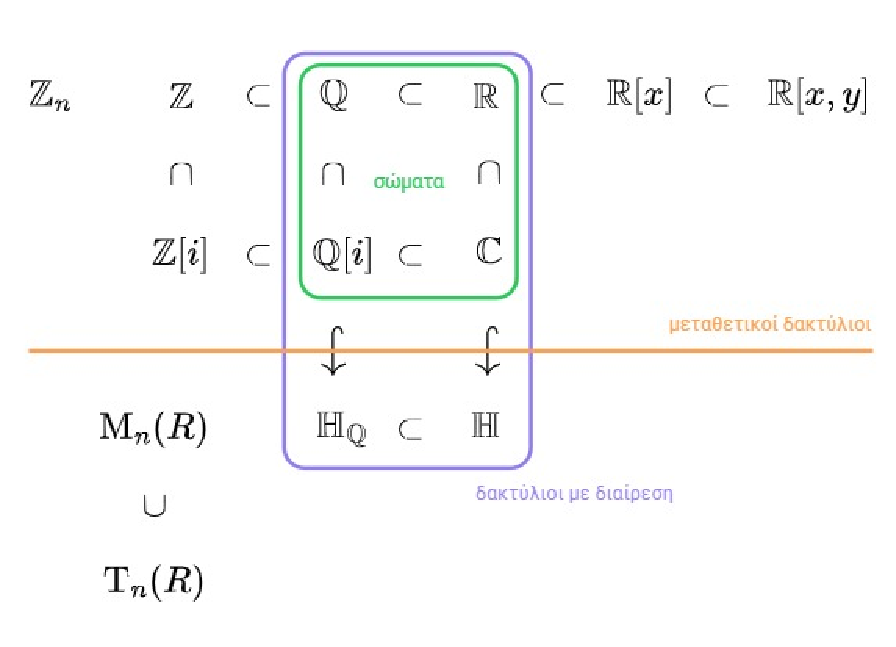
\includegraphics[width=0.6\textwidth]{rings_1.pdf}
    \vspace{-10pt} 
\end{figure}
όπου 
\begin{itemize}
    \item $\ZZ[i]$ και $\QQ[i]$ είναι ο δακτύλιος των ακεραίων και των ρητών του Gauss, αντίστοιχα,
    \item $\rmM_n(R)$ και $\rmT_n(R)$ είναι ο δακτύλιος των $(n\times{n})$-πινάκων και άνω τριγωνικών $(n\times{n})$-πινάκων με στοιχεία σε ένα δακτύλιο $R$, αντίστοιχα, και 
    \item $\HH$ είναι ο δακτύλιος των quaternions του Hamilton\footnote{Για μια γεωμετρική εξήγηση των quaternions του Hamilton δείτε \href{https://youtu.be/d4EgbgTm0Bg?si=wArxMheA85caUyqs}{εδώ}.} με στοιχεία (τυπικούς) γραμμικούς συνδυασμούς 
    \[
    a + bi + cj + dk
    \]
    στα σύμβολα $i, j, k$ και $a, b, c, d \in \CC$ με τον πολλαπλασιασμό να ικανοποιεί τους κανόνες 
    \begin{align*}
        i^2 &= j^2 = k^2 = -1 \\ 
        ij &= -ji = k \\
        jk &= -kj = i \\
        ki &= -ik = j.
    \end{align*}
\end{itemize}


\begin{remark}
    Το σύνολο $2\ZZ$ όλων των άρτιων ακεραίων ικανοποιεί όλες τις προϋποθέσεις του Ορισμού \ref{def:ring}, πλήν του αξιώματος (6), καθώς \emph{δεν} είναι εφοδιασμένος με μονάδα. Κατά συνέπεια, για το μάθημα αυτό, δεν το θεωρούμε δακτύλιο. Αυτό που εμείς αποκαλούμε δακτύλιο γενικότερα ονομάζεται \emph{δακτύλιος με μονάδα} (unital ring ή ring with identity).
\end{remark}

Μπουρούμε να φανταστούμε ένα(ν μεταθετικό) δακτύλιο ως ένα αφηρημένο \textquote{αριθμητικό σύστημα}, στο οποίο μπορούμε να κάνουμε \textquote{αριθμητική}. Για παράδειγμα,
\begin{itemize}
    \item το άθροισμα (αντ. γινόμενο) ενός πεπερασμένου πλήθους στοιχείων είναι καλώς ορισμένο\footnote{Στην περίπτωση που έχουμε έναν μη μεταθετικό δακτύλιο πρέπει να είμαστε πιο προσεκτικοί, καθώς γινόμενα της μορφής $\prod_{a \in X}a$ για κάποιο $X\subseteq R$ δεν είναι καλώς ορισμένα.}
    \item η αφαίρεση συμπεριφέρεται με τον αναμενόμενο τρόπο
    \item έχουμε βαθμωτό πολλαπλασιασμό\footnote{Το σύμβολο $\coloneqq$ σημαίνει \textquote{εξ' ορισμού}.}
    \[
    n a \coloneq
    \begin{cases}
        \underbrace{a + a + \cdots + a}_{\text{$n$ φορές}}, &\ \text{αν $n > 0$} \\
        -(\underbrace{a + a + \cdots + a}_{\text{$n$ φορές}}), &\ \text{αν $n < 0$}
    \end{cases}
    \]
    για κάθε $n \in \ZZ$, όπου $0_\ZZ a \coloneqq 0_R$
    \item μπορούμε να ορίσουμε δυνάμεις 
    \[
    a^n \coloneq \underbrace{a\cdot a \cdot \cdots \cdot a}_{\text{$n$ φορές}}
    \]
    για κάθε $n \in \ZZ$, όπου $a^{0_\ZZ} \coloneqq 1_R$
\end{itemize}
(βλ. \cite[Πρόταση~7.1.4]{Mpe15}).

Από την άλλη μεριά, πρέπει να είμαστε προσεκτικοί, διότι κάποια πράγματα δε δουλεύουν όπως θα περιμέναμε. Για παράδειγμα, 
\[
2 \cdot 3 = 6 \equiv 0 \pmod{6}.
\]
Κατά συνέπεια, για κάποιες τιμές του $n$ στον δακτύλιο $\ZZ_n$ το γινόμενο δύο μη μηδενικών στοιχείων \emph{δεν} είναι κατά ανάγκη μη μηδενικό.

\begin{definition}
    \label{def:zero_divisor_integral_domain}
    Έστω $R$ ένας δακτύλιος. Ένα μη μηδενικό $a \in R$ ονομάζεται \defn{μηδενοδιαιρέτης} (zero divisor) αν υπάρχει μη μηδενικό $b \in R$ τέτοιο ώστε 
    \[
    a \cdot b = 0 \quad \text{ή} \quad b \cdot a = 0.
    \]
    Ένα μεταθετικός δακτύλιος χωρίς μηδενοδιαιρέτες ονομάζεται \defn{ακέραια περιοχή} (integral domain).
\end{definition}

Αν ο $n$ είναι σύνθετος, δηλαδή $n = k\ell$ για κάποιους θετικούς ακεραίους $k, \ell$, τότε ο $\ZZ_n$ δεν μπορεί να είναι ακέραια περιοχή, διότι 
\[
k \cdot \ell = n \equiv 0 \pmod{n}.
\]
Για την ακρίβεια, το $\ZZ_n$ είναι ακέραια περιοχή αν και μόνο αν ο $n$ είναι πρώτος. Γενικότερα, κάθε ακέραια περιοχή με πεπερασμένο πλήθος στοιχείων είναι σώμα (βλ. \cite[Πρόταση~7.4.13]{Mpe15}). Μπορούμε να εμπλουτίσουμε έτσι το διάγραμμα παραδειγμάτων που είδαμε παραπάνω:
\begin{figure}[h]
    \centering
    \vspace{-12pt}
    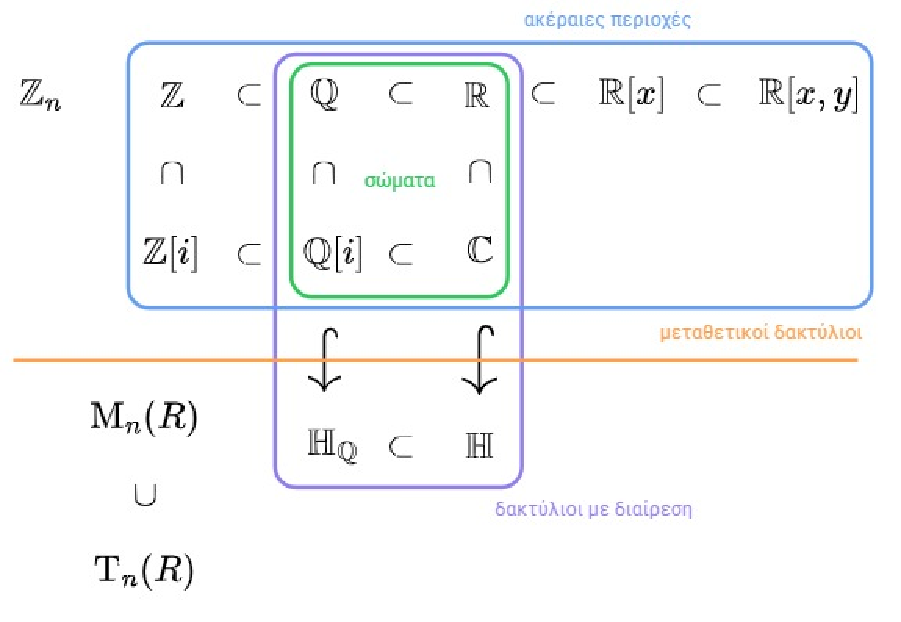
\includegraphics[width=0.6\textwidth]{rings_2.pdf} 
    \vspace{-10pt} 
\end{figure}

\begin{definition}
    \label{def:subring}
    Έστω $R$ ένας δακτύλιος. Ένα υποσύνολο $S \subseteq R$ ονομάζεται \defn{υποδακτύλιος} του $R$ αν 
    \begin{itemize}
        \item περιέχει το μηδέν και την μονάδα του $R$ 
        \item είναι κλειστό ως προς 
            \begin{itemize}
                \item την πρόσθεση, δηλαδή 
                \[
                a \in S \ \ \text{και} \ \ b \in S \quad \then \quad a+b \in S
                \]
                \item  τον πολλαπλασιασμό, δηλαδή
                \[
                a \in S \ \ \text{και} \ \ b \in S \quad \then \quad a\cdot b \in S
                \]
                \item αντίθετα στοιχεία, δηλαδή  
                \[
                a \in S \quad \then \quad -a \in S.
                \]
            \end{itemize}
    \end{itemize}
\end{definition}

Παρατηρήστε ότι στο διάγραμμα παραδειγμάτων οι δακτύλιοι που βρίσκονται αριστερά και πάνω από τα σύμβολα $\subset$ ικανοποιούν τα αξιώματα του Ορισμού \ref{def:subring}.

\begin{definition}
    \label{def:ring_homomorphism}
    Έστω $R$ και $S$ δύο δακτύλιοι. Μια απεικόνιση $\phi : R \to S$ ονομάζεται \defn{ομομορφισμός δακτυλίων} αν 
    \begin{itemize}
        \item διατηρεί το μηδέν και την μονάδα, δηλαδή 
        \[
        \phi(0_R) = 0_S \quad \text{και} \quad \phi(1_R) = 1_S
        \]
        \item διατηρεί την πρόσθεση, δηλαδή 
        \[
        \phi(a+b) = \phi(a) + \phi(b) 
        \]
        \item διατηρεί τον πολλαπλασιασμό, δηλαδή 
        \[
        \phi(a\cdot b) = \phi(a)\cdot\phi(b).
        \]
    \end{itemize}
    Ένας ομομορφισμός δακτυλίων ο οποίος είναι 1-1 και επί ονομάζεται \defn{ισομορφισμός} και στην περίπτωση αυτή γράφουμε $R \cong S$. Tέλος, το σύνολο 
    \[
    \ker\phi \coloneqq \{a \in R : \phi(a) = 0_S\}
    \]
    ονομάζεται \defn{πυρήνας} (kernel) του ομομορφισμού $\phi$.
\end{definition}

Για παράδειγμα, η απεικόνιση 
\begin{align*}
    \pi : \ZZ &\to \ZZ_n \\ 
    a &\mapsto a \pmod{n}
\end{align*}
είναι ομομορφισμός δακτυλίων με πυρήνα 
\begin{align*}
    \ker\phi 
    &= \{a \in \ZZ : \pi(a) = 0_{\ZZ_n}\} \\
    &= \{a \in \ZZ : a \equiv 0 \pmod{n}\} \\
    &= \{a \in \ZZ : n \vert a\} \\
    &\coloneqq n\ZZ.
\end{align*}

Στην παρατήρηση μετά τον Ορισμό \ref{def:ring} είδαμε ότι το $n\ZZ$ δεν αποτελεί δακτύλιο. Συνεπώς, ο πυρήνας $\ker\phi$ ενός ομομορφισμού δακτυλίων $\phi: R \to S$ δεν είναι (κατ' ανάγκη) υποδακτύλιος του $R$. Από την άλλη μεριά, η εικόνα
\[
\phi(R) \coloneqq \{b \in S : b = \phi(a), \ \text{για κάποιο $a \in R$}\}
\]
είναι υποδακτύλιος του $S$ (γιατί;). Στο προηγούμενο παράδειγμα έχουμε $\pi(\ZZ) = \ZZ_n$.

Ένα μη-παράδειγμα ομομορφισμού δακτυλίων είναι η απεικόνιση 
\begin{align*}
    \ZZ &\to \ZZ \\
    a &\mapsto na
\end{align*}
για κάθε $n > 1$, διότι δεν διατηρεί την μονάδα.

\begin{thebibliography}{99}
    \bibitem{Mpe15}
    Α. Μπελιγιάννης, 
    \textit{Μια Εισαγωγή στη Βασική Άλγεβρα},
    Κάλλιπος, 2015. (διαθέσιμο \href{https://dx.doi.org/10.57713/kallipos-547}{εδώ})
\end{thebibliography}
\end{document}